\documentclass[a4paper,12pt]{report}
\usepackage[english]{babel} % en
\usepackage{graphicx}
\usepackage{hyperref}
\usepackage[T1]{fontenc}
\usepackage[utf8]{inputenc}
\usepackage{setspace}
\usepackage[paper=a4paper,margin=1in]{geometry}
\usepackage{parskip}
\usepackage{fancyhdr}
\usepackage[superscript]{cite}
\usepackage{units}
\usepackage[htt]{hyphenat}
\usepackage{enumitem}
\usepackage{wrapfig}
\usepackage{mathtools}
\pagestyle{fancy}

\begin{document}
	
	\begin{titlepage}
		
		\begin{minipage}[t]{0.19\textwidth}
			\vspace{-4mm}{
\includegraphics[scale=1.15]{images/logo_unimib.pdf}}
		\end{minipage}
		\begin{minipage}[t]{0.81\textwidth}
			{
				\setstretch{1.42}
				{\textsc{Università degli Studi di Milano - Bicocca}} \\
				\textbf{Scuola di Scienze} \\
				\textbf{Dipartimento di Informatica, Sistemistica e Comunicazione} \\
				\textbf{Corso di laurea in Informatica} \\
				\par
			}
		\end{minipage}
		
		\vspace{40mm}
		
		\begin{center}
			{\LARGE{
					\setstretch{1.2}
					\textbf{A Data Analytics Framework for \\Medical Prescription Pattern Dynamics}
					\par
			}}
		\end{center}
		
		\vspace{40mm}
		
		{\large \textbf{Relatore:} Prof. Francesco Archetti} \\
		
		{\large \textbf{Correlatore:} Prof. Antonio Candelieri} \\
		
		{\large \textbf{Tutor aziendale:} Dott. Gaia Arosio} \\
		
		\vspace{15mm}
		
		\begin{flushright}
			{\large \textbf{Relazione della prova finale di:}} \\
			\large{Ilaria Battiston} \\
			\large{Matricola 816339} 
		\end{flushright}
		
		\vspace{30mm}
		\begin{center}
			{\large{\bf Anno Accademico 2018-2019}}
		\end{center}
		
		\restoregeometry
		
	\end{titlepage}
    
\newpage
\begin{abstract}
	Research on prescription pattern dynamics exploits medical information to highlight the issues concerning the growing antibiotic resistance among the Italian country, using a subset of data regarding the Campania region.
	
	After a clear understanding of the problem and the available information, along with its quality and feasible outcomes, a first analytical approach allows reconstruction of diagnosis and prescriptions global trending, from which is possible to extract patient journeys and underline changes.
	
	A deeper insight on antibiotics verifies national studies on overprescription, giving additional information on general practitioners' behaviour, brands popularity and seasonality of prescriptions, obtained with time series analysis and clustering.
\end{abstract}
\newpage
\setcounter{tocdepth}{1}
\tableofcontents
\newpage
\chapter{Introduction}
\section{Antibiotic resistance and misuse}
Antimicrobial resistance is a rising global problem which threatens the effective prevention and treatment of an ever-increasing range of infections caused by bacteria, parasites, viruses and fungi\cite{who}. 

Microorganisms exposed to antimicrobial drugs develop the ability to defeat substances designed to kill them, making infections persist in the body due to the unsuccessful action of agents.

This issue threatens public health causing higher healthcare costs to treat patients, and potentially compromising surgeries and chemotherapy results due to the ineffectiveness of antibiotics. No one can completely avoid the risk of resistant infections, but some people are at greater risk than others (for example, people with chronic illnesses)\cite{cdc}.

Antimicrobial resistance occurs naturally over time, usually through genetic changes. However, \textbf{the misuse and overuse of antimicrobials is accelerating this process}. In many places, antibiotics are overused and misused in people and animals, and often given without professional oversight\cite{who}.

Infections such as the common cold or sore throats are often countered with antibiotics, which have no effect against viruses and could as well put patients at the risk of suffering adverse reaction\cite{bmj}.

Therefore, to minimise the development of resistance, contributing factors must be reduced, optimising the use of drugs. This work requires effective surveillance and follow-up of consumption, at a local and national level. 

To be effective in the long run, work to optimise use of antibiotics must influence the prescribing practices of individual physicians. The goal is “rational use”, i.e. the correct patient receives the correct antibiotic at the correct dose and for the correct duration of treatment, in accordance with evidence-based guidelines. Over-prescribing should be avoided without resulting in under-prescribing\cite{sweden}.

Such work should be carried out close to the prescriber, something which also requires high resolution prescription data, down to the clinic and health centre level or better still at the level of \textbf{individual prescribers}.

\section{National Sanitary Service in Italy} % finire
The Italian National Sanitary Service (SSN) consists the complex of functions, activities and healthcare services offered by the State. It is based on subsidiarity, a general principle of the European Union law, stating that a central authority should have a subsidiary function, performing only those tasks which cannot be performed at a more local level\cite{oxford}.

SSN is articulated in different responsibility levels divided among the State, Regions, institutions and organisations, along with private structures and the Health Ministry, which coordinates the national sanitary plan.

Citizens benefit of healthcare services paying a related ticket\cite{ticket}, which represents the established way to contribute to expenses. It is used for:
\begin{itemize}
	\item Specialist examinations;
	\item First-aid help in non-emergency situations;
	\item Thermal care.
\end{itemize}

General practitioners' visits are exempted from payment of tickets. 
% tickets, ruolo del medico di base (prescrive le ricette) in modo generico, tanto c'è scritto dopo

\subsection{Drugs and prescriptions}
% AIFA
% prescrizioni di farmaci etici (scenario, evoluzione del settore) 30 pagine
%Rapporti di farmindustria, siti ministero Salute, agenas, federfarma

From the year 2000 every form of participation to sanitary expenses from citizens has been abolished\cite{ticket}, yet most Regions have introduced special drugs classes with a fixed quota for each medical prescription or package, to remedy the economic deficit. 

% le classi di farmaci sono: a, h, ???

% farmaci generci

\subsection{Antibiotic resistance in Italy}

\section{Healthcare data}
%dati, collezione, come sono raccolti, open data in italia, società (aicuvia oims health), promofarma (farmacisti, organizza informaticamente i dati e li vende → aziende farmaceutiche), agenzia delle entrate (codice fiscale), spiegare come sono organizzati ecc
%3) proprietari sistemi sw di medicina generale, millennium
%3 canali di produzione del dato (medici, farmacisti, ae) + canale derivato aicuvia

\section{Data classification}
% idc9, atc, etc

\section{Healthcare analytics}
\textbf{Healthcare analytics} is a field of growing importance which allows a deep understanding of results collected in the healthcare area. 

Extracting insights can be a complex challenge: health big data gives a huge \textit{volume} and \textit{variety} of information, therefore accessing the resources in a quick way is necessary. 

Other issues to deal with are \textit{veracity}, \textit{validity} and \textit{viability}, fundamental characteristics to ensure reliable and relevant analytics. Checking for integrity and quality can be difficult to verify without domain knowledge\cite{4vs}.

One of the various applications of this field is the change of patterns in the historical data: this research specifically focuses on \textbf{prescription pattern changes} on chronic patients, highlighting the development of some common medicines through time.

The considered healthcare data is a dump of a database created and handled by Millennium Srl\cite{millewin}, a leader company in IT services for medicine. This has been obtained through an extraction procedure on the original DB, assigning unique names to each table and column.

There are five main necessary fields for analysis\cite{DC}:
\begin{enumerate}
	\item \textbf{Spatial data}, in different granularity levels;
	\item \textbf{Personal data} of patients;
	\item \textbf{Temporal data}, in a range from 2000 to 2018, for time-series analysis;
	\item \textbf{Pharmacotherapeutic data}, classifiable according to different identification codes;
	\item \textbf{Diagnostic data}, for cross-validation of diagnoses.
\end{enumerate}

The two main risks encountered while doing analysis are information loss and inappropriate prescribing, that compromise the quality of statistics. Data may be incomplete, biased or filled with noise: another goal of analytics is to contrast incompleteness and incorrectness, obtaining coherent and clear results.

\chapter{Goals definition} % finire da qui
\section{Methodologies}
A general practitioner can do a wide range of daily activities, consisting in:
\begin{itemize}
	\item 
\end{itemize}
This specifical research is focussed on doctor-patient relationships, in particular information concerning diagnoses and prescriptions and their changes according to habits, time and geographical area. 

The dataset is modelled in a relational schema, which allows organization of records in structures (tables) to maintain integrity and compatibility between different kind of fields. For a better fruition of the workload, table names have been changed to standard English keywords.




%Relazione, modello ER, db stratificato, soglia temporale (dati disponibili & usati: avvento del generico, 10 anni)
%Funnel, perdita progressiva di informazioni, aree individuate, patologie (atc, prodotti), analisi globali 

\section{Considerations}
Since health big data can provide a high variety of information, it is required to have some clear \textit{objectives} in mind to keep on track and avoid losing focus. 

The research is centred on the \textbf{changes of prescription patterns of antibiotics}: this is a wide goal, and more information is needed to achieve results. It's necessary to narrow the field down, only concentrating on some classes of medicines, and define subgroups of GPs and patients in a restricted amount of time.

To obtain constraints the more objective as possible, some further analysis can be useful. For instance, focussing on chronic patients is a relatively fast way to reduce the huge amount of rows to elaborate, but causes the loss of most information.

The first step to take, having a deep understanding of the data, is recognising the extent and impact of the \textbf{progressive information loss}, to define the final amount of clear records. Trying to fix mistakes is a risk, since the outcome could be incorrect, so deleting is the most practical option.

Removing unclear and futile data may not be enough to have consistent results: 18 years of data is a wide range, and \textit{splitting the dataset} or deciding to only consider a smaller scope can be beneficial for the analysis quality. 

Some constraints can be imposed on general practitioners as well: since the results have to be coherent and accurate, it's best practice to only consider \textbf{active GPs} with a \textbf{constant number of patients} (to be defined). \\ This would partially remedy the fact that doctors may have different approaches to the same disease.

The creation of cohorts (chronic patients) among the statistical population is an example of \textbf{cluster sampling}.

After the initial parsing, there will be a rough draft of the final result which then will be subject of the following steps:
\begin{enumerate}
	\item Further analysis on data correctness (record linkage);
	\item Elaboration of the statistics and time series clustering.
\end{enumerate}

Another relevant instance for analysis is the \textbf{subset} of diseases to consider: choices have to be made according to \textit{external studies}, \textit{marketing researches} and further \textit{discoveries on the provided data}. Focussing on the \textbf{most common ones} is a guideline to start.

Having an idea of which illnesses and prescription have unstable patterns might give a better vision, and can be done through statistics on the whole database. 

Some examples of analytics are:
\begin{itemize}
	\item Most common diseases through the years;
	\item Most common \textit{chronic} diseases through the years;
	\item Changes of the number of prescriptions for diseases in the same area;
	\item Changes of prescriptions based on the patient phenotype or market trends.
\end{itemize}

An obstacle to perceiving the meaning of results is the restricted domain knowledge: to compensate, confronting some experts in the field is required. The team comprehends computer scientists, statisticians, biologists and healthcare workers.

% spostare
The tools to analyse and elaborate the health data are:
\begin{itemize}
	\item \textbf{PostgreSQL}, for data management and querying;
		\begin{itemize}
			\item The software project to interface with the web server is \textbf{PgAdmin 4};
			\item All queries need to be optimized to avoid huge computational times, using indexes and Common Table Expressions;
		\end{itemize}
	\item \textbf{R}, for machine learning and graphics computing;
	\begin{itemize}
		\item There are many ways to create plots;
		\item Possible uses are time series analysis and trajectory clustering.
	\end{itemize}
\end{itemize}

Reports and slide-shares have been created and accessed using the \textbf{Google Suite}.

Due to the amount of sensitive data, detailed results are going to be omitted: the final conclusions will be a product of aggregation and schematisation.

\section{Practical goals}
 
\chapter{Data description}

\section{Overview of the database}
The database used for analytics contains data on medical histories of patients between \textbf{January 2000} and \textbf{October 2018.} 

It's important to note that the research work has been done on only a part of the whole database, consisting in \textbf{5 tables}. There is information available on \textbf{general practitioners}, \textbf{patients}, \textbf{diagnoses} and \textbf{prescriptions}: each macro-category is included in a separated table, so it's necessary to recognise the relationship between fields.

The 5 tables and their relative sizes are:
\begin{itemize}
	\item \textit{pazienti}, 1.015.618 tuples; \\
	Basic information about patients, identified by an encrypted UID;
	\item \textit{nos\_002}, 1.015.618 tuples; \\
	Extension of \textit{pazienti} with the same key, containing more detailed information and linkage with GPs;
	\item \textit{cart\_pazpbl}, 15.460.199 tuples; \\
	Information about diagnoses and relative description;
	\item \textit{cart\_terap}, 118.716.403 tuples; \\
	Information about therapies and prescribed medicines;
	\item \textit{cart\_accert}, 151.478.456 tuples; \\
	Information about medical checks and examinations.
\end{itemize}

It's easy to see that the number of rows is varying a lot: there are a lot more prescriptions than diagnosis, and 150 millions of medical examinations. 

Each diagnosis, prescription and examination is uniquely distinguished by the triplet patient-GP-date, which maps to \textit{codice--userid--time\_last} in the database. 

There are many other date fields, but \textit{time\_last} (last update of the record) is the only one of type \textit{timestamp}, making each one different from the others (it's unlikely to have a diagnosis or prescription for the same patient, by the same doctor and at the same exact moment). 

Analysis is performed using dates in the \textit{YYYY-MM-DD} format, since there's no need of unique data: there are lots of different prescription for the same patient made on the same day.

\section{Description of the tables}
Below is reported a brief description of the 5 tables, along with the main fields used for analytics and their meaning.

\subsection{\textit{pazienti}}
The table \textit{pazienti} includes information about patients. To maintain privacy, there are no real names: everything is \textbf{encrypted} as a 22-character string containing letters, numbers and special symbols.

Other relevant fields are:
\begin{itemize}
	\item \textit{data\_open}, date of beginning of the doctor-patient relationship;
	\item \textit{nascita}, date of birth;
	\item \textit{decesso}, eventual date of death;
	\item \textit{comune\_di\_nascita}, name (and code) of the birth municipality;
	\item \textit{sesso}, birth sex;
	\item \textit{pa\_convenzione}, type of convention with the Italian insurance system.
\end{itemize}

\subsection{\textit{nos\_002}}
The table \textit{nos\_002} contains the same information as \textit{pazienti}, with additional fields which are essential to analyse data:
\begin{itemize}
	\item \textit{pa\_medi}, \textbf{encrypted} UID of the general practitioner of the patient;
	\item \textit{pa\_cap}, zip-code of the patient (for geographical analysis);
	\item \textit{pa\_pro}, province of the patient;
	\item \textit{pa\_drevoca}, eventual date of termination of the doctor-patient relationship (a patient changing GP).
\end{itemize}

All the IDs of the GPs, along with all other data on GPs, are stored in an external table \textit{users} (the research has been made considering a subset of the original DB). The latter will be used to identify active doctors, but doesn't contain any other useful information.

\subsection{\textit{cart\_pazpbl}}
The table \textit{cart\_pazpbl} comprehends the diagnoses associated to patients and relative GPs. Each diagnosis is defined by its \textbf{ICD-9} code, an international identifier for diseases maintained by the World Health Organization. 

Fields summary:
\begin{itemize}
	\item \textit{codice}, patient ID;
	\item \textit{userid}, corresponding to \textit{pa\_medi }in \textit{nos\_002 }(general practitioner ID);
	\item \textit{data\_open}, date of insertion of the diagnosis in the database;
	\item \textit{time\_last}, timestamp of last edit of the tuple;
	\item \textit{nome\_pbl}, a textual description of the diagnosis;
	\item \textit{cp\_code}, code of the diagnosis according to the ICD-9 standards.
\end{itemize}

\subsection{\textit{cart\_terap}}
The table \textit{cart\_terap} contains the prescribed medicines for each patient. There is no linkage between diagnosis and prescriptions in the database, so additional work is required to detect correlation.

Each prescription is defined by an\textbf{ ATC code}, from the Anatomical Therapeutical Chemical classification system maintained by the World Health Organization. Furthermore, there are \textbf{active principle code} and \textbf{authorisation for commerce code}.

Fields summary:
\begin{itemize}
	\item \textit{codice}, patient ID;
	\item \textit{userid}, corresponding to \textit{pa\_medi }in \textit{nos\_002} (general practitioner ID);
	\item \textit{data\_open}, date of insertion of the prescription in the database;
	\item \textit{time\_last}, timestamp of last edit of the tuple;
	\item \textit{co\_codifa}, AIC code (authorisation for commerce);
	\item \textit{co\_des}, textual description of the medicine;
	\item \textit{te\_npezzi}, number of boxes;
	\item \textit{te\_attivo}, active principle code;
	\item \textit{co\_atc}, ATC code;
	\item \textit{euro}, price.
\end{itemize}

\subsection{\textit{cart\_accert}}
The table \textit{cart\_accert} includes all the medical checks and examination for each patient. The first goals of the research only included diagnoses and prescriptions, hence why the comprehension of this table isn't as deep as the others.

Each examination is defined by an \textbf{ICD-9-CM} code, an extension of the ICD-9 database with standard procedures. 

Fields summary:
\begin{itemize}
	\item \textit{codice}, patient ID;
	\item \textit{userid}, corresponding to \textit{pa\_medi} in \textit{nos\_002} (general practitioner ID);
	\item \textit{data\_open}, date of insertion of the examination in the database;
	\item \textit{time\_last}, timestamp of last edit of the tuple;
	\item \textit{ac\_nt\_code}, ICD-9-CM code;
	\item \textit{ac\_des}, textual description;
	\item \textit{cod\_ese}, exemption code for the examination.
\end{itemize}

\section{ER model}
After identifying the main fields, it's useful to build and include an \textbf{ER model}\cite{draw} to have a better understanding of the tables and their relationship.
\begin{figure}[h]
	\centering
	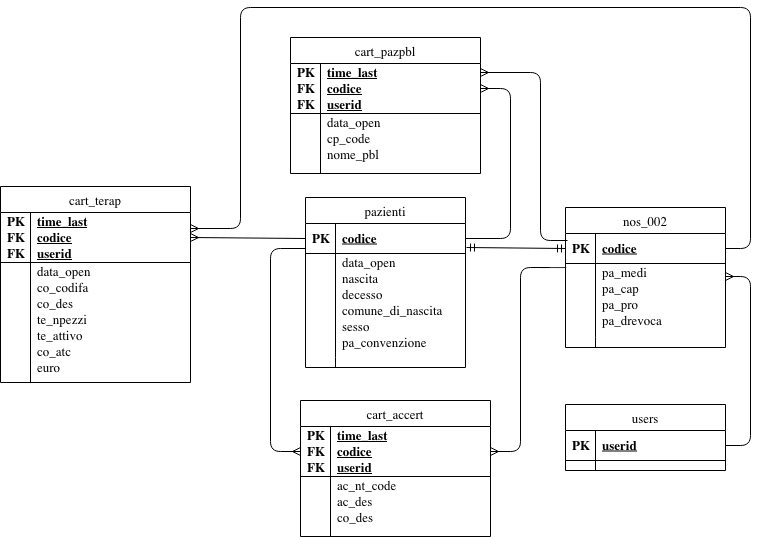
\includegraphics[scale=0.6]{immagini/er.png}
\end{figure}


\chapter{Information loss} 
This chapter aims to give a qualitative assessment of the whole database through an initial analysis, giving an overall idea on how impactful is the progressive information loss. 

After assessing the correctness and completeness of records, some fields will be eventually excluded from the analysis, while others that cannot be removed will have a major impact on the results.

Having missing fields, particularly in the process of joining tables, can lead to a \textbf{cumulative augmentation} of the information loss: empty data such as the patient date of birth or gender will cause the deletion of the entire patient, in case analytics is centred on pathologies by age or gender.

Joining is in fact an operation which requires \textit{all fields of reference to be present}, combining entries of the selected tables.

\section{General overview}
Before starting running queries, there are some aspects to consider involving issues which sometimes cannot be addressed just with database interrogations:
\begin{enumerate}
	\item The geographic information is sometimes imprecise and hard to comprehend, since it consists in text fields;
	\item Some diagnoses descriptions don't match with the corresponding ICD-9 code;
	\item A consistent amount of missing data is originated in case a general practitioner doesn't prescribe anything but makes other operations (medical certificates, examinations and such);
	\item Hospital prescriptions are missing;
	\item Some medicines are given over the counter without requiring a prescription, therefore there is no entry in the DB;
	\item General practitioners might prescribe a medicine to a different patient than the one who has the pathology (relatives, friends, \dots);
	\item There is inappropriate prescribing, antibiotic resistance, misuse or over-use of medicines;
	\item A patient can change doctor, so the approach to the same disease may vary.
\end{enumerate}

Furthermore, there have been noticed some common instances of incorrect data:
\begin{itemize}
	\item Some dates don't fall in the acceptable range (e.g.\ 1999, 2034, \dots):
	\begin{itemize}
		\item A date is considered wrong if it falls before 01-01-2000 or after 10-01-2018;
	\end{itemize}
	\item A consistent amount of fields are empty or null.
\end{itemize}

It is important to remember that some records might be affected by more than one incorrect field, therefore when calculating total information loss it is essential to intersect different subsets, to see which records they have in common, instead of just summing the numbers of corrupted rows.

Overall, the loss on single records is not a relevant issue since the total amount of rows allows safe removal, yet the cumulative augmentation (funnel analysis) gives a progressive deletion of information.

\section{Information loss on records}

\subsection{\textit{patients} and \textit{patient\_doctors} (1 million of tuples)}
\subsubsection{Summary}
Both tables contain similar data related to patients, with a $1 : 1$ correspondence between primary keys, therefore joining is an elementary operation and there is no information loss.

\begin{itemize}
	\item Patients with null or empty gender: 2 752 $\rightarrow 0.27\%$;
	\item Patients with gender different from M and F: 54 $\rightarrow 0.005\%$;
	\item Patients with beginning of the patient-doctor relationship outside the accepted range: 226 858 $\rightarrow 22.33\%$;
	\item Patients with null province: 99 981 $\rightarrow 9.84\%$.
\end{itemize}

A subset of patients is creating through an auxiliary view to highlight the final progressive data loss compared to the original tables, joining \textit{patients} and \textit{patients\_doctors} according to those constraints:
\begin{enumerate}
	\item Join on equal patient code (\textit{id});
	\item Not null date of birth;
	\item Dates between 2000 and 2018;
	\item Existing and not null gender;
	\item Existing and not null province.
\end{enumerate}

The total rows respecting all those constraints are 713 352, so approximatively 300 000 tuples (patients) have been deleted. 

This result implies that during analysis there will be at least $\nicefrac{1}{3}$ of the data which is going to be removed due to incompleteness and inaccuracy: not considering patients will imply deleting their diagnoses and prescriptions as well.

A waffle chart is shown on figure \ref{waffle}, highlighting the total tuples and the impact of every restriction, standardised on a scale from 1 to 100:
\begin{figure}[h]
	\centering
	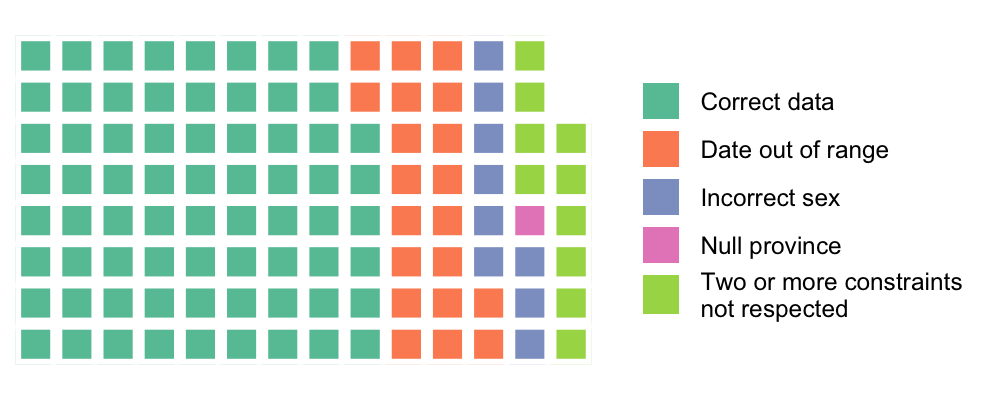
\includegraphics[scale=0.45]{../plots/patients-waffle.png}
	\caption{\small Information loss on patients, waffle plot}
	\label{waffle}
\end{figure}

There are no null provinces and birthdates. The bigger impact is caused by dates falling outside the acceptable range, meaning patients started treatment with their general practitioner earlier than 2000.

\subsection{\textit{diagnoses} (15 millions of tuples)}
\subsubsection{ICD-9}
An ICD-9 code is correct if it is present in the official ICD-9 database\cite{icd9}. General practitioners may use different formats and notations, so before removing codes each one has been subject to preprocessing and parsing.

An ICD-9 code is considered wrong if there is no match in the official DB after any of those transformations:
\begin{enumerate}
	\item Removal of the dot;
	\item Addition of 0 at the beginning;
	\item Addition of 0 at the end;
	\item Removal of the last 0.
\end{enumerate}

There are 76 distinct incorrect ICD-9 codes, a negligible amount considering the total records consisting in 9 895 distinct codes.

\subsubsection{Summary}
\begin{itemize}
	\item Incorrect ICD-9 codes: $76 \rightarrow 0.0005\%$;
	\item Null or empty ICD-9 codes: 2 103 169 $\rightarrow 13.02\%$;
	\item Null or empty descriptions: 656 067 $\rightarrow 4.24\%$;
	\item Dates out of range: 807 985 $\rightarrow 5.23\%$.
\end{itemize}

Empty descriptions almost always correspond to empty ICD-9 codes, therefore the total information loss on descriptions is absorbed by null codes, resulting in the same 13.02\% united percentage.

\subsection{\textit{prescriptions} (118 millions of tuples)}
\subsubsection{ATC code}
The ATC code, unlike ICD-9, has a univocal format (a numeric string of 7 digits), and no parsing is needed. All the codes have been checked with the ontologies in a well-known biology portal\cite{atc}, and an ATC is considered incorrect if there is no match.

There are 1 750 292 non-existent codes, which are caused by:
\begin{enumerate}
	\item Alteration of the codes within the years without updating the database;
	\item Single prescriptions indexed using the superclass code;
	\item Codes only recognised by local pharmacies.
\end{enumerate}

The latter is the most common reason: there are up to 90 000 occurrences of a single unofficial code. Those numbers, despite being high, are not majorly impacting results, considering the total amount of 118 millions of records.

\subsubsection{Summary}
\begin{itemize}
	\item Incorrect ATC codes: 1 750 292 $\rightarrow 1.47\%$;
	\item Null or empty ATC codes: 1 577 749 $\rightarrow 1.33\%$;
	\item Null or empty AIC codes: 1 310 719 $\rightarrow 1.1\%$;
	\item Null or empty descriptions: 101 248 410 $\rightarrow 85.28\%$;
	\item Dates out of range: 3 472 119 $\rightarrow 2.92\%$.
\end{itemize}

Clearly, the prescription description is not a field which can be used for reliable analytics since empty values prevail.

The field \textit{pieces} (number of boxes) might be useful to check for appropriate prescribing, but since the field is a string it requires casting and parsing to integer, and it could be more relevant to focus on prescription patterns.

\section{Total information loss}
Overall, total information loss is shown according by its belonging table. 

\begin{table}[!htb]
	
	\centering
	\begin{minipage}[c]{0.4\linewidth}
				\begin{tabular}{c|c|c}
				\textbf{Table} & \textbf{Records} & \textbf{Percentage} \\
				\hline
				\textit{patients} & 302 266 & 29\% \\
				\hline
				\textit{diagnoses} & 2 403 202 & 15.5\% \\
				\hline
				\textit{prescriptions} & 5 560 191 & 4.7\& \\
			\end{tabular}
	\end{minipage}
	\qquad
	\begin{minipage}[c]{0.4\linewidth}
		\qquad
		\centering
		$\rightarrow$
		\qquad
		\begin{tabular}{c}
			\textbf{Usable records} \\
			\hline
			713 352 \\
			\hline
			13 056 997 \\
			\hline
			113 156 212 \\
		\end{tabular}
		
	\end{minipage}
	\caption{\small Information loss summary}
\end{table}



The aggregated results are not final: each single output from interrogations will be influenced by all the different invalid fields (i.\ e. a patient could have all correct data yet a missing prescription AIC), creating a progressive deletion effect.

Overall, percentages do not compose the majority of tuples, since tables have magnitude order of millions.


\chapter{Patient journey}
After the preliminary analysis and deciding the main focus area, there are enough information to begin reconstructing the \textbf{patient journey}. The goal of this process is to highlight changes in \textit{prescription patterns for chronic diseases}, starting from the medical history of patients.

An objective definition of patient journey can be created using the following guidelines:
\begin{enumerate}
	\item Patients with \textbf{complete medical history} for a fixed amount of years;
	\item Records with patient, prescribing GP, diagnosis and prescription on the \textbf{same date};
	\item Only \textbf{first-time }diagnoses and prescriptions considered.
\end{enumerate}

The imposed criteria is very strict: taking diagnoses and prescriptions on the same day means removing \textit{all prescriptions} following the first diagnosis. In other words, all the instances of patients coming back to their GP to renew a prescription for a chronic disease have been deleted.

This can be useful to extract a cohort of patients beginning their treatment, and analyse the variations of first-time prescriptions. It's important to notice that not all doctors may have patients with a new chronic illness.

\section{Imposed criteria}
Aside from the completeness and correctness of the data, there are more restrictions to maintain the consistency:
\begin{itemize}
	\item The prescribing general practitioner mustn't change in the time range;
	\item The patient mustn't be deceased;
	\item There must be a sanitary convention;
	\item The general practitioner must be active.
\end{itemize}

All those constraints can be checked using the related fields in the database: \textit{pa\_drevoca} for interruption of the relationship, \textit{decesso} for death and \textit{pa\_convenzione} for the sanitary convention.

The table \textit{users} contains all the IDs of active general practitioners, so joining it with other tables is enough to remove all the rows with an inactive GP. Data is up to date, but since the patient journey will include 2018 (the focus is on the most recent information) there is no need to check for active GPs in the previous years.

The biggest risk is again the \textbf{loss of information}: the impact of data cleansing is heavy, and the obtained results might not give an insightful prospective.

\section{Initial data cleaning}
An initial data cleaning has been made on the whole database to have a first understanding of the potential information loss.

In this case, having such a big amount of tuples is useful: it's possible to remove a considerable percentage of them without losing generality and still having numerous samples.

Information on the general loss is already available thanks to the specific analysis on each single field, so the shown data cleaning will only consider patients and GPs.

The active general practitioners are \textbf{432}: this result has been retrieved counting the different IDs in \textit{users} (438) and removing the ones that weren't present in \textit{nos\_002} (6).

The following \textit{pie chart} illustrates the data loss on patients according to the criteria defined in the previous section.
\begin{figure}[h]
	\centering
	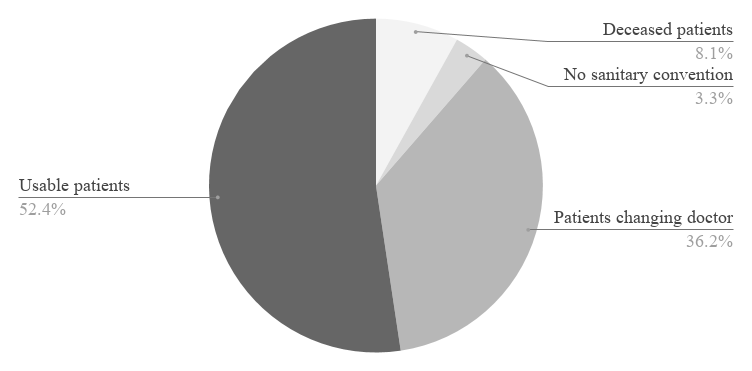
\includegraphics[scale=0.6]{images/pie0018.png}
\end{figure}

About half of patients is going to be lost, due to not respecting the consistency criteria. Starting from a million of records, concrete results are still obtainable.

\section{First approach}
The first approach consists in testing with an \textbf{arbitrary range constraint}: all dates must fall in the span between 2010 and 2018.

The analysis has pure research purposes, to understand the impact of a cut of the dataset in terms of information loss. All the previously introduced criteria must be considered as well, so there must be a continuous doctor-patient relationship between active GPs and non-deceased patients with sanitary conventions.

The outcome is a patient journey table containing data from 2000 to 2018, with a total amount of \textbf{144.618} tuples: this means that there are roughly 150k of first-time diagnosis and prescriptions to patients. 

\subsection{Results breakdown}
Seeing that the starting tables had number of rows in the order of millions, some deeper analysis is necessary to figure out the causes of this huge loss.

The 144.618 complete tuples are composed by:
\begin{itemize}
	\item 27.733 patients;
	\item 422 general practitioners;
	\item 1.381 unique diagnoses;
	\item 904 unique prescriptions.
\end{itemize}

Further causes for those low values can be found counting how many dates would not fall in the considered range. The percentage of records with date earlier than 2010 in each table is:
\begin{itemize}
	\item Patients: 75\%;
	\item Diagnosis: 54,6\%;
	\item Prescriptions: 44,7\%.
\end{itemize}

There is an enormous loss on patients: the possible reason might be that most patients started treatment earlier than 2010, plus diagnosis and relative prescription are in different dates.

8 years is a too wide range to obtain a consistent patient journey, and such information loss isn't negligible: the conclusion of the first approach is that introducing time boundaries is something which needs an accurate control, to avoid missing out most of the data.

\newpage
\section{Second approach}
Since just removing according to the date is an abrupt approach, it's necessary to tune parameters and introduce more detailed constraint, to have a bigger amount of information.

The focus is on the number of prescriptions: given a small range of years, only patients with at least one new prescription are going to be considered. All the previous criteria must be respected, so there must be a continuous doctor-patient relationship between active GPs and non-deceased patients with sanitary conventions.

This methodology allows cluster sampling without having to remove half of the dates: criteria based on the number of prescriptions creates another patient cohort which can be used to accurately select rows from the other tables.

The proposed time range is 2016-2018: pharmaceutical companies generally use the last two years of sales, so picking the last three years gives additional information without compromising the consistency of data.

The outcome is a patient journey consisting of 1.465.005 tuples: almost 10 times the previous result. This leads to two important statements:
\begin{enumerate}
	\item The time range is appropriate, since the number is large enough to make analysis without loss of generality;
	\item The new imposed criterion gives more consistent data and the possibility to build time series.
\end{enumerate}

More cleaning is required to link diagnoses and prescriptions, since there is not a 1:1 correspondence: multiple diagnosis and prescriptions may be associated to the same date. This can be done using a lookup table.

\subsection{Results breakdown}
The 1.665.005 complete tuples are composed by:
\begin{itemize}
	\item 230.381 patients;
	\item 422 general practitioners;
	\item 1.381 unique diagnoses;
	\item 904 unique prescriptions.
\end{itemize}

Only 7\% of the total prescription has been taken in consideration, yet a million and half is still a satisfying amount.

\section{Results comparison}
Comparing the two patient journey outcomes through graphs is a good way to visualize changes and improvements.

\subsection{Changes in data composition}
% todo

\subsection{Improvement on patients information loss}
% todo
A pie chart for data loss on patients in the range 2016-2018 has been made to compare with the previous one.

\begin{figure}[h]
	\centering
	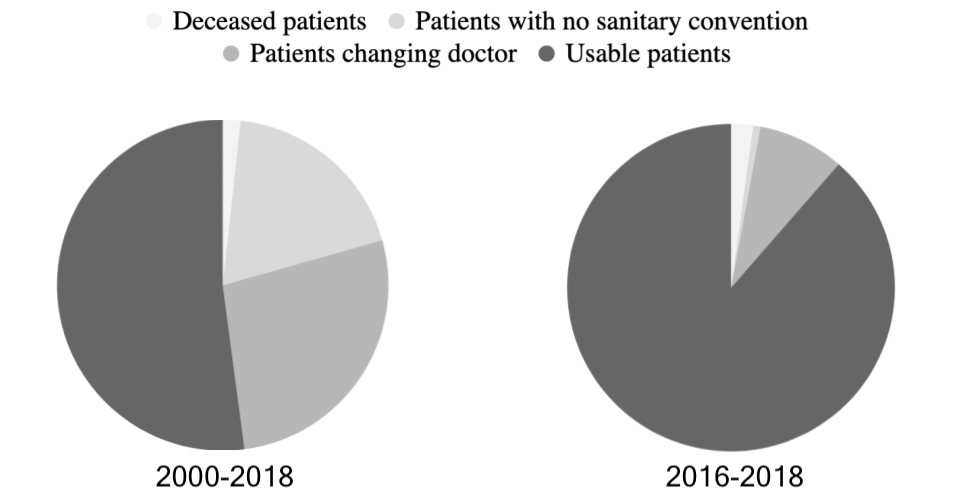
\includegraphics[scale=0.5]{images/pies.png}
\end{figure}

It's easy to see that the number of usable patients has noticeably increased: using a smaller time span reduces the chances of death and change of GP.

\subsection{Funnel graph of patients}
A funnel graph is useful to see how imposing every restriction made the patients number decrease: starting from a million, in the end there only is about $\nicefrac{1}{4}$ of it.








\begin{thebibliography}{}
	\footnotesize
	
	\bibitem{4vs}
	\texttt{https://healthitanalytics.com/news/understanding-the-many-vs-of-healthcare-big-data-analytics}
	
	\bibitem{millewin}
	\texttt{https://www.millewin.it/}
	
	\bibitem{generico}
	\texttt{https://www.normattiva.it/uri-res/N2Ls?urn:nir:stato:legge:1995-12-29;549~art3!vig=}
	
	\bibitem{aifaar}
	\texttt{http://www.agenziafarmaco.gov.it/content/la-resistenza-agli-antibiotici-emergenza-mondiale-il-primo-rapporto-globale-del-who}
	
	\bibitem{DC}
	Davide Castaldi, \textit{Richiesta Dati CNCM per Analisi Appropriatezza Prescrittiva}, Consorzio Milano Ricerche, 2018.
	
	\bibitem{draw}
	Made with \texttt{draw.io}.
	
	\bibitem{icd9}
	Manuale ICD-9-CM versione italiana 2007. \\
	\texttt{http://www.salute.gov.it/portale/documentazione/p6\_2\_2\_1.jsp?lingua=italiano\&id=2251}
	
	\bibitem{DC2}
	Davide Castaldi, \textit{Allegato Tech DB Campania}, Consorzio Milano Ricerche, 2018.
	
	\bibitem{atc}
	\texttt{https://bioportal.bioontology.org/ontologies/ATC} 
	
	\bibitem{medicinaliequivalenti}
	\texttt{http://www.agenziafarmaco.gov.it/sites/default/files/medicinali\_equivalenti-qualita\_sicurezza\_efficacia.pdf}
	
	\bibitem{wonca2}
	\texttt{https://www.woncaeurope.org/sites/default/files/documents/Definizione\%20WONCA\%202011\%20ita\_A4.pdf}
	
	\bibitem{pg}
	\texttt{https://www.postgresql.org/}
	
	\bibitem{neo}
	\texttt{https://neo4j.com/}
	
	\bibitem{r}
	\texttt{https://www.r-project.org/}
	
	\bibitem{who}
	\texttt{https://www.who.int/en/news-room/fact-sheets/detail/antimicrobial-resistance}
	
	\bibitem{cdc}
	\texttt{https://www.cdc.gov/drugresistance/about.html}
	
	\bibitem{sweden}
	\texttt{https://www.folkhalsomyndigheten.se/contentassets/dae82c7afd424a57b57ec81818793346/swedish-work-on-containment-of-antibiotic-resistance.pdf}
	
	\bibitem{bmj}
	\texttt{bmj.com/cgi/pmidlookup?view=long\&pmid=9270458}
	
	\bibitem{oxford}
	\texttt{https://en.oxforddictionaries.com/definition/subsidiarity}
	
	\bibitem{ticket}
	\texttt{http://www.salute.gov.it/portale/esenzioni/dettaglioContenutiEsenzioni.jsp?lingua=italiano\&id=4674\&area=esenzioni\&menu=vuoto}
	
	\bibitem{classi}
	\texttt{http://www.fcr.re.it/classificazione-dei-farmaci-ai-fini-della-rimborsabilita}
	
	\bibitem{ricette}
	\texttt{https://web.archive.org/web/20111129162006/http://www.farmaciadicello.it/ricetta-01.htm}
	
	\bibitem{wonca1}
	\texttt{https://web.archive.org/web/20140611065109/http://www.woncaeurope.org/sites/default/files/documents/Definition\%203rd\%20ed\%202011\%20with\%20revised\%20wonca\%20tree.pdf}
	
	\bibitem{gp}
	\texttt{http://www.salute.gov.it/portale/temi/p2\_6.jsp?lingua=italiano\&id=1698\&area=tumori\&menu=percorso}
	
	\bibitem{ascpt}
	\texttt{https://ascpt.onlinelibrary.wiley.com/doi/full/10.1038/clpt.2008.24}
	
	\bibitem{whoicd}
	\texttt{https://www.who.int/classifications/icd/en/}
	
	\bibitem{icdit}
	\texttt{http://www.salute.gov.it/portale/temi/p2\_6.jsp?lingua=italiano\&id=1982\&area=statisticheSSN\&menu=definizioni}
	
	\bibitem{icd9en}
	\texttt{https://www.medicalbillingandcodingonline.com/icd-cm-codes/}
	
	\bibitem{aicdef}
	\texttt{http://www.agenziafarmaco.gov.it/glossary/term/1432}
	
	\bibitem{aic}
	\texttt{http://www.agenziafarmaco.gov.it/content/l\%E2\%80\%99autorizzazione-all\%E2\%80\%99immissione-commercio}
	
	\bibitem{atclevels}
	\texttt{https://www.whocc.no/filearchive/publications/2019\_guidelines\_web.pdf}
	
	\bibitem{repubblica}
	\texttt{https://www.repubblica.it/salute/medicina-e-ricerca/2019/03/13/news/antibioticoresistenza\_in\_italia\_il\_primato\_europeo\_di\_decessi-221467306/}
	
	\bibitem{antibiotic}
	\texttt{https://www.medicalnewstoday.com/articles/10278.php}
	
	\bibitem{calo}
	\texttt{https://www.aboutpharma.com/blog/2019/01/10/antibiotici-continua-il-calo-della-ricerca-e-sviluppo-secondo-locse/}
	
	\bibitem{usa}
	\texttt{https://clincalc.com/DrugStats/Top300Drugs.aspx}
	
	\bibitem{bacteria}
	\texttt{https://www.infectioncontroltoday.com/antibiotics-antimicrobials/study-shows-antibiotics-destroy-immune-cells-and-worsen-oral-infection}
	
	\bibitem{dedalus}
	\texttt{https://www.dedalus.eu/}
	
	\bibitem{datapine}
	\texttt{https://www.datapine.com/blog/big-data-examples-in-healthcare/}
	
	\bibitem{bentelan}
	\texttt{https://www.my-personaltrainer.it/Foglietti-illustrativi/Bentelan.html}
	
	\bibitem{agenziafarmaco}
	\texttt{http://www.agenziafarmaco.gov.it/content/la-resistenza-agli-antibiotici-emergenza-mondiale-il-primo-rapporto-globale-del-who}
	
\end{thebibliography}
	

\end{document}